\documentclass{article}
\usepackage[utf8]{inputenc}
\usepackage[margin=1in]{geometry}

\title{485 - Homework 6}
\author{Victor Zhang}
\date{November 12, 2021}

\usepackage[utf8]{inputenc}
\usepackage{amsmath}
\usepackage{amsfonts}
\usepackage{natbib}
\usepackage{graphicx}
% \usepackage{changepage}
\usepackage{amssymb}
\usepackage{xfrac}
% \usepackage{bm}
% \usepackage{empheq}
\usepackage{subcaption}
\usepackage{hyperref}
\usepackage{cleveref}
\usepackage{svg}

\newcommand{\contra}{\raisebox{\depth}{\#}}

\newenvironment{myindentpar}[1]
  {\begin{list}{}
          {
            \setlength{\leftmargin}{#1}
            \setlength{\rightmargin}{#1}
          }
          \item[]
  }
  {\end{list}}

\pagestyle{empty}

\begin{document}

\maketitle
% \begin{center}
% {\huge Econ 482 \hspace{0.5cm} HW 3}\
% {\Large \textbf{Victor Zhang}}\
% {\Large February 18, 2020}
% \end{center}

\section{}
\subsection{}
By definition, $\Phi(Z) = U$, where $Z$ is the standard normal. Then $\Phi(\Phi^{-1}(U)) = U$ implies $\Phi^{-1}(U) \sim Z$ $\Box$

\subsection{}
\begin{figure}[ht!]
\begin{subfigure}[h]{0.3\linewidth}
  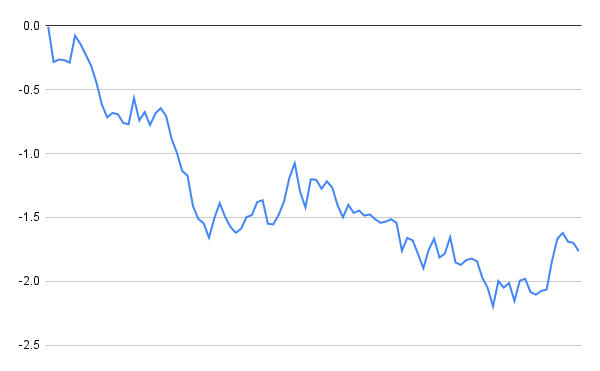
\includegraphics[width=\linewidth]{img/bm1.png}
  \caption{Brownian 1}
\end{subfigure}
\hfill
\begin{subfigure}[h]{0.3\linewidth}
  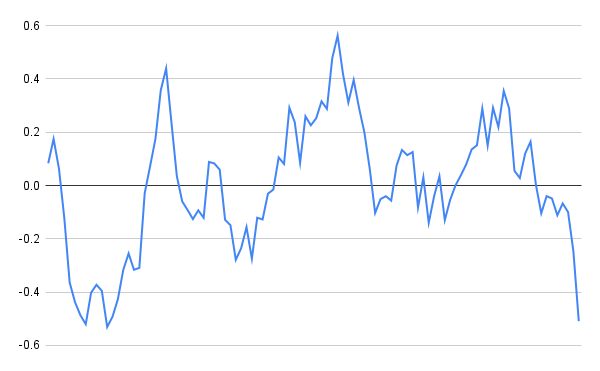
\includegraphics[width=\linewidth]{img/bm2.png}
  \caption{Brownian 2}
\end{subfigure}
\hfill
\begin{subfigure}[h]{0.3\linewidth}
  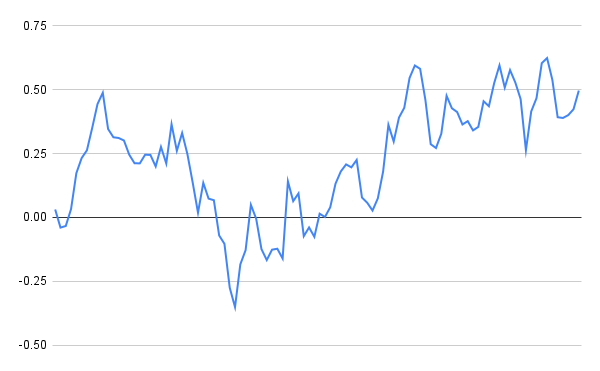
\includegraphics[width=\linewidth]{img/bm3.png}
  \caption{Brownian 3}
\end{subfigure}
\hfill
\end{figure}
\subsection{}
\begin{figure}[ht!]
\begin{subfigure}[h]{0.3\linewidth}
  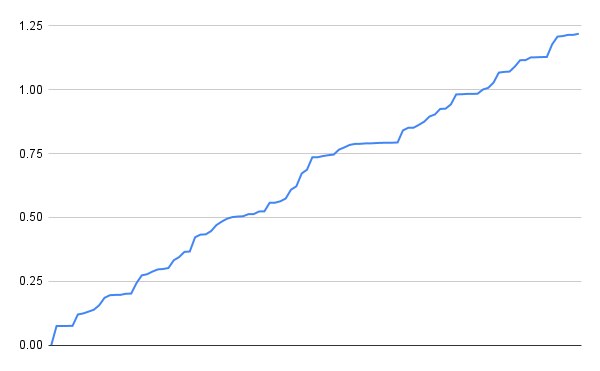
\includegraphics[width=\linewidth]{img/qv1.png}
  \caption{Brownian 1}
\end{subfigure}
\hfill
\begin{subfigure}[h]{0.3\linewidth}
  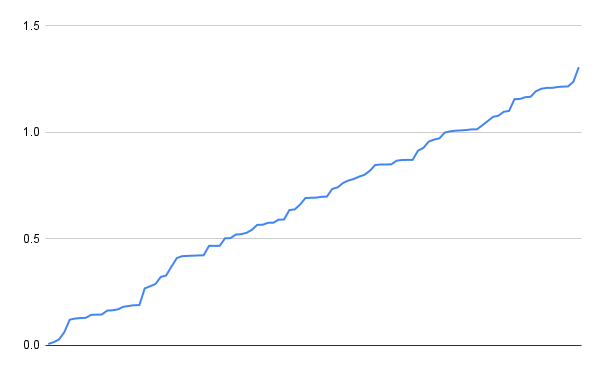
\includegraphics[width=\linewidth]{img/qv2.png}
  \caption{Brownian 2}
\end{subfigure}
\hfill
\begin{subfigure}[h]{0.3\linewidth}
  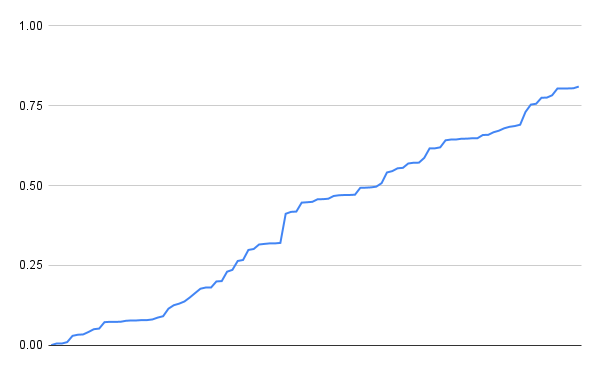
\includegraphics[width=\linewidth]{img/qv3.png}
  \caption{Brownian 3}
\end{subfigure}
\hfill
\end{figure}

\section{}
$$\mathbb{E} \left[ \sum_{n = 0}^{N - 1} (X_{t_{n+1}} - X_{t_n})(Y_{t_{n+1}} - Y_{t_n}) \right] = \sum_{n = 0}^{N - 1} \mathbb{E}[(B_{t_{n+1}} - B_{t_n})](t_{n+1} - t_n) = \sum_{n = 0}^{N - 1} 0 = 0 $$
\begin{equation*}
\begin{split}
\mathrm{var}\left( \sum_{n = 0}^{N - 1} (X_{t_{n+1}} - X_{t_n})(Y_{t_{n+1}} - Y_{t_n}) \right) &= \mathrm{var}\left( \sum_{n = 0}^{N - 1} (B_{t_{n+1}} - B_{t_n})(t_{n+1} - t_n) \right)\\
&= \sum_{n = 0}^{N - 1} \mathrm{var}\left( (B_{t_{n+1}} - B_{t_n})(t_{n+1} - t_n) \right)\\
&= \sum_{n = 0}^{N - 1} (t_{n+1} - t_n)^2 \mathrm{var}(B_{t_{n+1}} - B_{t_n})\\
&= \sum_{n = 0}^{N - 1} (t_{n+1} - t_n)^2 (t_{n+1} - t_n)\\
&= \sum_{n = 0}^{N - 1} T^3/N^3 = \frac{T^3}{N^2}
\end{split}
\end{equation*}
where we have used the independent increments property of Brownian motion to pass the variance into the sum.\\
Taking limit $|\Pi| \to 0$, $\mathbb{E}[[X,Y]_T] = 0$ and $\mathrm{var}([X,Y]_T) = 0$. By convergence in $L^2$, $[X,Y]_t = 0$ $\Box$

\section{}
For arbitrary $0 \leq s \leq t \leq T$,
\begin{equation*}
\begin{split}
\mathbb{E}_s[f(B_t^2)] &= \mathbb{E}_s[f((B_t - B_s + B_s)^2)]\\
&= \mathbb{E}_s[f((B_t - B_s)^2 + 2(B_t - B_s)B_s + B_s^2)]\\
\end{split}
\end{equation*}
We know $(B_t - B_s)^2$ and $(B_t - B_s)$ are independent of $\mathcal{F}_s$ so by independence lemma we may put
$$g(x) = \mathbb{E}[f((B_t - B_s)^2 + 2(B_t - B_s)x + x^2)]$$
so thus $B^2$ is Markov $\Box$

\section{}
$$\mathbb{E}_s \left[ \sum \Delta_j (B_{t_{j+1}} - B_{t_j}) \right] = \sum \mathbb{E}_s[\Delta_j(B_{t_{j+1}} - B_{t_j})]$$
Suppose $\Delta$ is simple. That is, $\Delta_j$ is constant on $[t_j, t_{j+1})$. Then by linearity of expectation, we may write $\mathbb{E}_j[\Delta_j(X)] = \Delta_j(\mathbb{E}_j[X])$.\\
For all $t_{j + 1} <= s$, $B_{j+1}, B_j$ are known so
$$\mathbb{E}_s[\Delta_j(B_{t_{j+1}} - B_{t_j})] = \Delta_j(B_{t_{j+1}} - B_{t_j}) = \Delta_j(B_{t_{j+1 \wedge s}} - B_{t_j \wedge s})$$
For $t_j > s$ we iterate
$$\mathbb{E}_s[\Delta_j(B_{t_{j+1}} - B_{t_j})] = \mathbb{E}_s[\Delta_j(\mathbb{E}_j[B_{t_{j+1}} - B_{t_j}])] = \Delta_j(0) = \Delta_j(B_{t_{j+1 \wedge s}} - B_{t_j \wedge s})$$
For the case $t_j \leq s < t_{j + 1}$ we note
$$\mathbb{E}_s[\Delta_j(B_{t_{j+1}} - B_{t_j})] = \Delta_j(\mathbb{E}_s[B_{t_{j+1}} - B_{t_j}]) = \Delta_j(B_s - B_{t_j}) = \Delta_j(B_{t_{j+1 \wedge s}} - B_{t_j \wedge s})$$
So the statement is proven for simple $\Delta$.\\
To prove the statement for general $\Delta$, we appeal to the construction of the Lebesgue integral and dominated convergence $\Box$

\end{document}

% List of tex snippets:
%   - tex-header (this)
%   - R      --> \mathbb{R}
%   - Z      --> \mathbb{Z}
%   - B      --> \mathcal{B}
%   - E      --> \mathbb{E}
%   - M      --> \mathcal{M}
%   - m      --> \mathfrak{m}({#1})
%   - normlp --> \norm{{#1}}_{L^{{#2}}}
